\documentclass[1p]{elsarticle_modified}
%\bibliographystyle{elsarticle-num}

%\usepackage[colorlinks]{hyperref}
%\usepackage{abbrmath_seonhwa} %\Abb, \Ascr, \Acal ,\Abf, \Afrak
\usepackage{amsfonts}
\usepackage{amssymb}
\usepackage{amsmath}
\usepackage{amsthm}
\usepackage{scalefnt}
\usepackage{amsbsy}
\usepackage{kotex}
\usepackage{caption}
\usepackage{subfig}
\usepackage{color}
\usepackage{graphicx}
\usepackage{xcolor} %% white, black, red, green, blue, cyan, magenta, yellow
\usepackage{float}
\usepackage{setspace}
\usepackage{hyperref}

\usepackage{tikz}
\usetikzlibrary{arrows}

\usepackage{multirow}
\usepackage{array} % fixed length table
\usepackage{hhline}

%%%%%%%%%%%%%%%%%%%%%
\makeatletter
\renewcommand*\env@matrix[1][\arraystretch]{%
	\edef\arraystretch{#1}%
	\hskip -\arraycolsep
	\let\@ifnextchar\new@ifnextchar
	\array{*\c@MaxMatrixCols c}}
\makeatother %https://tex.stackexchange.com/questions/14071/how-can-i-increase-the-line-spacing-in-a-matrix
%%%%%%%%%%%%%%%

\usepackage[normalem]{ulem}

\newcommand{\msout}[1]{\ifmmode\text{\sout{\ensuremath{#1}}}\else\sout{#1}\fi}
%SOURCE: \msout is \stkout macro in https://tex.stackexchange.com/questions/20609/strikeout-in-math-mode

\newcommand{\cancel}[1]{
	\ifmmode
	{\color{red}\msout{#1}}
	\else
	{\color{red}\sout{#1}}
	\fi
}

\newcommand{\add}[1]{
	{\color{blue}\uwave{#1}}
}

\newcommand{\replace}[2]{
	\ifmmode
	{\color{red}\msout{#1}}{\color{blue}\uwave{#2}}
	\else
	{\color{red}\sout{#1}}{\color{blue}\uwave{#2}}
	\fi
}

\newcommand{\Sol}{\mathcal{S}} %segment
\newcommand{\D}{D} %diagram
\newcommand{\A}{\mathcal{A}} %arc


%%%%%%%%%%%%%%%%%%%%%%%%%%%%%5 test

\def\sl{\operatorname{\textup{SL}}(2,\Cbb)}
\def\psl{\operatorname{\textup{PSL}}(2,\Cbb)}
\def\quan{\mkern 1mu \triangleright \mkern 1mu}

\theoremstyle{definition}
\newtheorem{thm}{Theorem}[section]
\newtheorem{prop}[thm]{Proposition}
\newtheorem{lem}[thm]{Lemma}
\newtheorem{ques}[thm]{Question}
\newtheorem{cor}[thm]{Corollary}
\newtheorem{defn}[thm]{Definition}
\newtheorem{exam}[thm]{Example}
\newtheorem{rmk}[thm]{Remark}
\newtheorem{alg}[thm]{Algorithm}

\newcommand{\I}{\sqrt{-1}}
\begin{document}

%\begin{frontmatter}
%
%\title{Boundary parabolic representations of knots up to 8 crossings}
%
%%% Group authors per affiliation:
%\author{Yunhi Cho} 
%\address{Department of Mathematics, University of Seoul, Seoul, Korea}
%\ead{yhcho@uos.ac.kr}
%
%
%\author{Seonhwa Kim} %\fnref{s_kim}}
%\address{Center for Geometry and Physics, Institute for Basic Science, Pohang, 37673, Korea}
%\ead{ryeona17@ibs.re.kr}
%
%\author{Hyuk Kim}
%\address{Department of Mathematical Sciences, Seoul National University, Seoul 08826, Korea}
%\ead{hyukkim@snu.ac.kr}
%
%\author{Seokbeom Yoon}
%\address{Department of Mathematical Sciences, Seoul National University, Seoul, 08826,  Korea}
%\ead{sbyoon15@snu.ac.kr}
%
%\begin{abstract}
%We find all boundary parabolic representation of knots up to 8 crossings.
%
%\end{abstract}
%\begin{keyword}
%    \MSC[2010] 57M25 
%\end{keyword}
%
%\end{frontmatter}

%\linenumbers
%\tableofcontents
%
\newcommand\colored[1]{\textcolor{white}{\rule[-0.35ex]{0.8em}{1.4ex}}\kern-0.8em\color{red} #1}%
%\newcommand\colored[1]{\textcolor{white}{ #1}\kern-2.17ex	\textcolor{white}{ #1}\kern-1.81ex	\textcolor{white}{ #1}\kern-2.15ex\color{red}#1	}

{\Large $\underline{12a_{1274}~(K12a_{1274})}$}

\setlength{\tabcolsep}{10pt}
\renewcommand{\arraystretch}{1.6}
\vspace{1cm}\begin{tabular}{m{100pt}>{\centering\arraybackslash}m{274pt}}
\multirow{5}{120pt}{
	\centering
	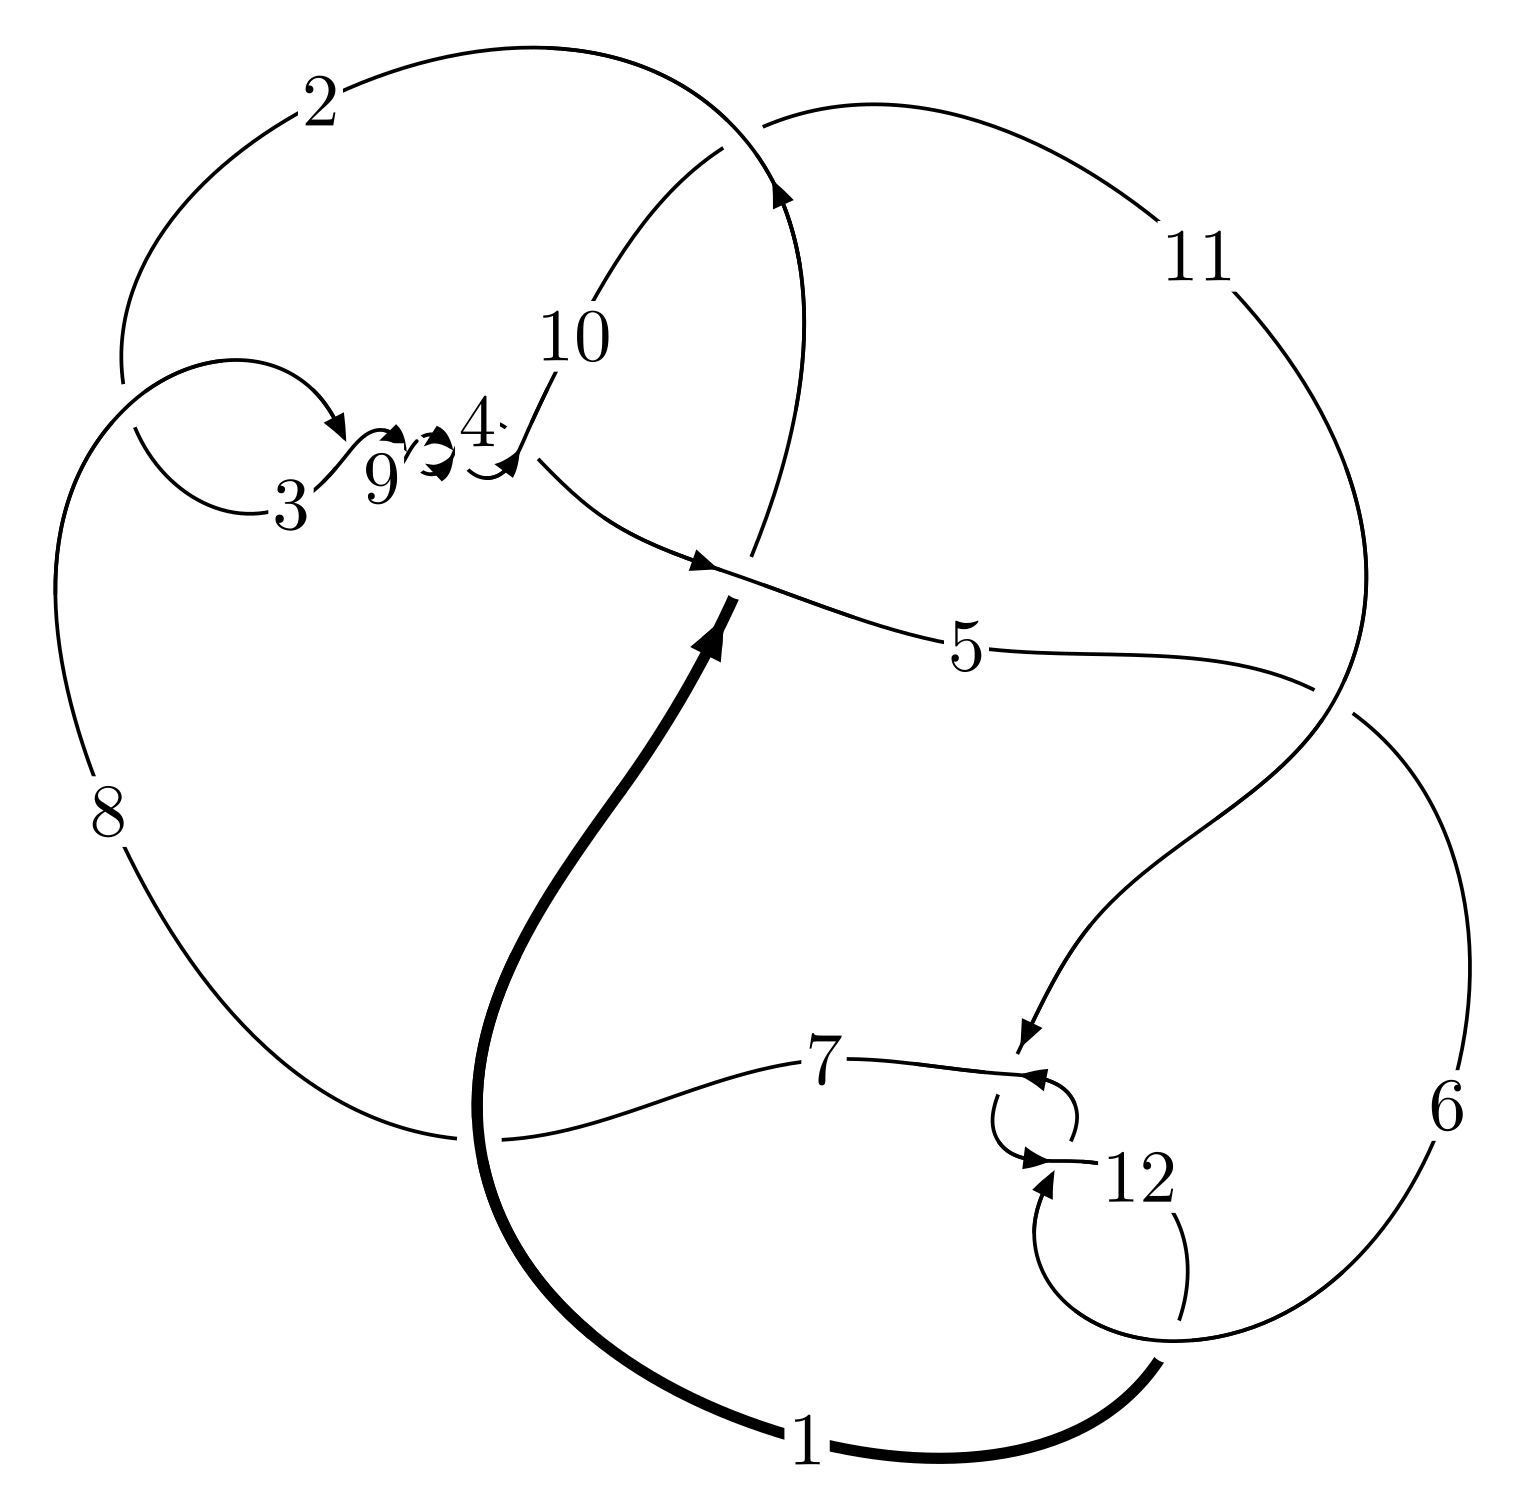
\includegraphics[width=112pt]{../../../GIT/diagram.site/Diagrams/png/2075_12a_1274.png}\\
\ \ \ A knot diagram\footnotemark}&
\allowdisplaybreaks
\textbf{Linearized knot diagam} \\
\cline{2-2}
 &
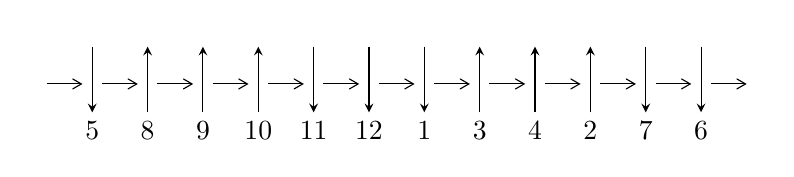
\begin{tikzpicture}[x=20pt, y=17pt]
	% nodes
	\node (C0) at (0, 0) {};
	\node (C1) at (1, 0) {};
	\node (C1U) at (1, +1) {};
	\node (C1D) at (1, -1) {5};

	\node (C2) at (2, 0) {};
	\node (C2U) at (2, +1) {};
	\node (C2D) at (2, -1) {8};

	\node (C3) at (3, 0) {};
	\node (C3U) at (3, +1) {};
	\node (C3D) at (3, -1) {9};

	\node (C4) at (4, 0) {};
	\node (C4U) at (4, +1) {};
	\node (C4D) at (4, -1) {10};

	\node (C5) at (5, 0) {};
	\node (C5U) at (5, +1) {};
	\node (C5D) at (5, -1) {11};

	\node (C6) at (6, 0) {};
	\node (C6U) at (6, +1) {};
	\node (C6D) at (6, -1) {12};

	\node (C7) at (7, 0) {};
	\node (C7U) at (7, +1) {};
	\node (C7D) at (7, -1) {1};

	\node (C8) at (8, 0) {};
	\node (C8U) at (8, +1) {};
	\node (C8D) at (8, -1) {3};

	\node (C9) at (9, 0) {};
	\node (C9U) at (9, +1) {};
	\node (C9D) at (9, -1) {4};

	\node (C10) at (10, 0) {};
	\node (C10U) at (10, +1) {};
	\node (C10D) at (10, -1) {2};

	\node (C11) at (11, 0) {};
	\node (C11U) at (11, +1) {};
	\node (C11D) at (11, -1) {7};

	\node (C12) at (12, 0) {};
	\node (C12U) at (12, +1) {};
	\node (C12D) at (12, -1) {6};
	\node (C13) at (13, 0) {};

	% arrows
	\draw[->,>={angle 60}]
	(C0) edge (C1) (C1) edge (C2) (C2) edge (C3) (C3) edge (C4) (C4) edge (C5) (C5) edge (C6) (C6) edge (C7) (C7) edge (C8) (C8) edge (C9) (C9) edge (C10) (C10) edge (C11) (C11) edge (C12) (C12) edge (C13) ;	\draw[->,>=stealth]
	(C1U) edge (C1D) (C2D) edge (C2U) (C3D) edge (C3U) (C4D) edge (C4U) (C5U) edge (C5D) (C6U) edge (C6D) (C7U) edge (C7D) (C8D) edge (C8U) (C9D) edge (C9U) (C10D) edge (C10U) (C11U) edge (C11D) (C12U) edge (C12D) ;
	\end{tikzpicture} \\
\hhline{~~} \\& 
\textbf{Solving Sequence} \\ \cline{2-2} 
 &
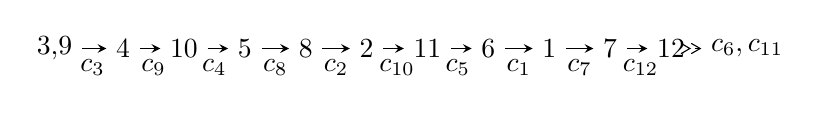
\begin{tikzpicture}[x=22pt, y=7pt]
	% node
	\node (A0) at (-1/8, 0) {3,9};
	\node (A1) at (1, 0) {4};
	\node (A2) at (2, 0) {10};
	\node (A3) at (3, 0) {5};
	\node (A4) at (4, 0) {8};
	\node (A5) at (5, 0) {2};
	\node (A6) at (6, 0) {11};
	\node (A7) at (7, 0) {6};
	\node (A8) at (8, 0) {1};
	\node (A9) at (9, 0) {7};
	\node (A10) at (10, 0) {12};
	\node (C1) at (1/2, -1) {$c_{3}$};
	\node (C2) at (3/2, -1) {$c_{9}$};
	\node (C3) at (5/2, -1) {$c_{4}$};
	\node (C4) at (7/2, -1) {$c_{8}$};
	\node (C5) at (9/2, -1) {$c_{2}$};
	\node (C6) at (11/2, -1) {$c_{10}$};
	\node (C7) at (13/2, -1) {$c_{5}$};
	\node (C8) at (15/2, -1) {$c_{1}$};
	\node (C9) at (17/2, -1) {$c_{7}$};
	\node (C10) at (19/2, -1) {$c_{12}$};
	\node (A11) at (45/4, 0) {$c_{6},c_{11}$};

	% edge
	\draw[->,>=stealth]	
	(A0) edge (A1) (A1) edge (A2) (A2) edge (A3) (A3) edge (A4) (A4) edge (A5) (A5) edge (A6) (A6) edge (A7) (A7) edge (A8) (A8) edge (A9) (A9) edge (A10) ;
	\draw[->>,>={angle 60}]	
	(A10) edge (A11);
\end{tikzpicture} \\ 

\end{tabular} \\

\footnotetext{
The image of knot diagram is generated by the software ``\textbf{Draw programme}" developed by Andrew Bartholomew(\url{http://www.layer8.co.uk/maths/draw/index.htm\#Running-draw}), where we modified some parts for our purpose(\url{https://github.com/CATsTAILs/LinksPainter}).
}\phantom \\ \newline 
\centering \textbf{Ideals for irreducible components\footnotemark of $X_{\text{par}}$} 
 
\begin{align*}
I^u_{1}&=\langle 
u^{47}- u^{46}+\cdots+2 u-1\rangle \\
\\
\end{align*}
\raggedright * 1 irreducible components of $\dim_{\mathbb{C}}=0$, with total 47 representations.\\
\footnotetext{All coefficients of polynomials are rational numbers. But the coefficients are sometimes approximated in decimal forms when there is not enough margin.}
\newpage
\renewcommand{\arraystretch}{1}
\centering \section*{I. $I^u_{1}= \langle u^{47}- u^{46}+\cdots+2 u-1 \rangle$}
\flushleft \textbf{(i) Arc colorings}\\
\begin{tabular}{m{7pt} m{180pt} m{7pt} m{180pt} }
\flushright $a_{3}=$&$\begin{pmatrix}1\\0\end{pmatrix}$ \\
\flushright $a_{9}=$&$\begin{pmatrix}0\\u\end{pmatrix}$ \\
\flushright $a_{4}=$&$\begin{pmatrix}1\\- u^2\end{pmatrix}$ \\
\flushright $a_{10}=$&$\begin{pmatrix}u\\- u^3+u\end{pmatrix}$ \\
\flushright $a_{5}=$&$\begin{pmatrix}- u^2+1\\u^4-2 u^2\end{pmatrix}$ \\
\flushright $a_{8}=$&$\begin{pmatrix}- u\\u\end{pmatrix}$ \\
\flushright $a_{2}=$&$\begin{pmatrix}- u^2+1\\u^2\end{pmatrix}$ \\
\flushright $a_{11}=$&$\begin{pmatrix}- u^7+4 u^5-4 u^3+2 u\\u^7-3 u^5+u\end{pmatrix}$ \\
\flushright $a_{6}=$&$\begin{pmatrix}- u^{18}+11 u^{16}-48 u^{14}+107 u^{12}-133 u^{10}+95 u^8-34 u^6+2 u^4+u^2+1\\u^{18}-10 u^{16}+37 u^{14}-60 u^{12}+35 u^{10}+8 u^8-16 u^6+4 u^4- u^2\end{pmatrix}$ \\
\flushright $a_{1}=$&$\begin{pmatrix}- u^8+5 u^6-7 u^4+2 u^2+1\\u^{10}-6 u^8+11 u^6-6 u^4+u^2\end{pmatrix}$ \\
\flushright $a_{7}=$&$\begin{pmatrix}- u^{19}+12 u^{17}-58 u^{15}+144 u^{13}-193 u^{11}+130 u^9-26 u^7-14 u^5+5 u^3\\u^{21}-13 u^{19}+\cdots+u^3+u\end{pmatrix}$ \\
\flushright $a_{12}=$&$\begin{pmatrix}u^{46}-29 u^{44}+\cdots+4 u^2+1\\- u^{46}+28 u^{44}+\cdots-8 u^4+u^2\end{pmatrix}$\\&\end{tabular}
\flushleft \textbf{(ii) Obstruction class $= -1$}\\~\\
\flushleft \textbf{(iii) Cusp Shapes $= -4 u^{44}+116 u^{42}+\cdots-20 u+6$}\\~\\
\newpage\renewcommand{\arraystretch}{1}
\flushleft \textbf{(iv) u-Polynomials at the component}\newline \\
\begin{tabular}{m{50pt}|m{274pt}}
Crossings & \hspace{64pt}u-Polynomials at each crossing \\
\hline $$\begin{aligned}c_{1}\end{aligned}$$&$\begin{aligned}
&u^{47}+7 u^{46}+\cdots+64 u+23
\end{aligned}$\\
\hline $$\begin{aligned}c_{2},c_{3},c_{4}\\c_{8},c_{9}\end{aligned}$$&$\begin{aligned}
&u^{47}- u^{46}+\cdots+2 u-1
\end{aligned}$\\
\hline $$\begin{aligned}c_{5},c_{7}\end{aligned}$$&$\begin{aligned}
&u^{47}+u^{46}+\cdots-22 u-13
\end{aligned}$\\
\hline $$\begin{aligned}c_{6},c_{11},c_{12}\end{aligned}$$&$\begin{aligned}
&u^{47}- u^{46}+\cdots-2 u^2-1
\end{aligned}$\\
\hline $$\begin{aligned}c_{10}\end{aligned}$$&$\begin{aligned}
&u^{47}-5 u^{46}+\cdots+56 u-16
\end{aligned}$\\
\hline
\end{tabular}\\~\\
\newpage\renewcommand{\arraystretch}{1}
\flushleft \textbf{(v) Riley Polynomials at the component}\newline \\
\begin{tabular}{m{50pt}|m{274pt}}
Crossings & \hspace{64pt}Riley Polynomials at each crossing \\
\hline $$\begin{aligned}c_{1}\end{aligned}$$&$\begin{aligned}
&y^{47}+11 y^{46}+\cdots-9704 y-529
\end{aligned}$\\
\hline $$\begin{aligned}c_{2},c_{3},c_{4}\\c_{8},c_{9}\end{aligned}$$&$\begin{aligned}
&y^{47}-61 y^{46}+\cdots-4 y-1
\end{aligned}$\\
\hline $$\begin{aligned}c_{5},c_{7}\end{aligned}$$&$\begin{aligned}
&y^{47}-29 y^{46}+\cdots-1076 y-169
\end{aligned}$\\
\hline $$\begin{aligned}c_{6},c_{11},c_{12}\end{aligned}$$&$\begin{aligned}
&y^{47}+39 y^{46}+\cdots-4 y-1
\end{aligned}$\\
\hline $$\begin{aligned}c_{10}\end{aligned}$$&$\begin{aligned}
&y^{47}-5 y^{46}+\cdots+6176 y-256
\end{aligned}$\\
\hline
\end{tabular}\\~\\
\newpage\flushleft \textbf{(vi) Complex Volumes and Cusp Shapes}
$$\begin{array}{c|c|c}  
\text{Solutions to }I^u_{1}& \I (\text{vol} + \sqrt{-1}CS) & \text{Cusp shape}\\
 \hline 
\begin{aligned}
u &= -0.935316 + 0.305335 I\end{aligned}
 & \phantom{-}2.62027 - 2.29094 I & \phantom{-}4.17636 + 2.98224 I \\ \hline\begin{aligned}
u &= -0.935316 - 0.305335 I\end{aligned}
 & \phantom{-}2.62027 + 2.29094 I & \phantom{-}4.17636 - 2.98224 I \\ \hline\begin{aligned}
u &= \phantom{-}0.966803 + 0.319748 I\end{aligned}
 & -0.38211 + 6.33274 I & \phantom{-}1.15955 - 6.71320 I \\ \hline\begin{aligned}
u &= \phantom{-}0.966803 - 0.319748 I\end{aligned}
 & -0.38211 - 6.33274 I & \phantom{-}1.15955 + 6.71320 I \\ \hline\begin{aligned}
u &= -0.952629 + 0.220168 I\end{aligned}
 & \phantom{-}3.38277 - 2.89354 I & \phantom{-}6.69037 + 6.29889 I \\ \hline\begin{aligned}
u &= -0.952629 - 0.220168 I\end{aligned}
 & \phantom{-}3.38277 + 2.89354 I & \phantom{-}6.69037 - 6.29889 I \\ \hline\begin{aligned}
u &= -0.985625 + 0.326270 I\end{aligned}
 & \phantom{-}4.24927 - 10.39780 I & \phantom{-}5.89159 + 8.40345 I \\ \hline\begin{aligned}
u &= -0.985625 - 0.326270 I\end{aligned}
 & \phantom{-}4.24927 + 10.39780 I & \phantom{-}5.89159 - 8.40345 I \\ \hline\begin{aligned}
u &= \phantom{-}0.948541 + 0.084215 I\end{aligned}
 & \phantom{-}2.09196 + 0.10474 I & \phantom{-}3.38715 + 0.99978 I \\ \hline\begin{aligned}
u &= \phantom{-}0.948541 - 0.084215 I\end{aligned}
 & \phantom{-}2.09196 - 0.10474 I & \phantom{-}3.38715 - 0.99978 I \\ \hline\begin{aligned}
u &= \phantom{-}1.021670 + 0.243299 I\end{aligned}
 & \phantom{-}9.32278 + 3.73916 I & \phantom{-}10.74415 - 4.44796 I \\ \hline\begin{aligned}
u &= \phantom{-}1.021670 - 0.243299 I\end{aligned}
 & \phantom{-}9.32278 - 3.73916 I & \phantom{-}10.74415 + 4.44796 I \\ \hline\begin{aligned}
u &= -1.053170 + 0.103400 I\end{aligned}
 & \phantom{-}6.61499 + 3.02641 I & \phantom{-}9.00744 - 2.18164 I \\ \hline\begin{aligned}
u &= -1.053170 - 0.103400 I\end{aligned}
 & \phantom{-}6.61499 - 3.02641 I & \phantom{-}9.00744 + 2.18164 I \\ \hline\begin{aligned}
u &= \phantom{-}0.641912 + 0.301512 I\end{aligned}
 & \phantom{-}0.98188 + 3.42521 I & \phantom{-}2.41709 - 5.44099 I \\ \hline\begin{aligned}
u &= \phantom{-}0.641912 - 0.301512 I\end{aligned}
 & \phantom{-}0.98188 - 3.42521 I & \phantom{-}2.41709 + 5.44099 I \\ \hline\begin{aligned}
u &= -0.560169 + 0.321250 I\end{aligned}
 & -2.59632 + 0.42907 I & -1.68504 + 1.57161 I \\ \hline\begin{aligned}
u &= -0.560169 - 0.321250 I\end{aligned}
 & -2.59632 - 0.42907 I & -1.68504 - 1.57161 I \\ \hline\begin{aligned}
u &= \phantom{-}0.511129 + 0.368669 I\end{aligned}
 & \phantom{-}1.68279 - 4.29871 I & \phantom{-}3.25946 + 0.95874 I \\ \hline\begin{aligned}
u &= \phantom{-}0.511129 - 0.368669 I\end{aligned}
 & \phantom{-}1.68279 + 4.29871 I & \phantom{-}3.25946 - 0.95874 I \\ \hline\begin{aligned}
u &= \phantom{-}0.187143 + 0.547043 I\end{aligned}
 & \phantom{-}0.63696 + 7.42810 I & \phantom{-}0.40676 - 7.42331 I \\ \hline\begin{aligned}
u &= \phantom{-}0.187143 - 0.547043 I\end{aligned}
 & \phantom{-}0.63696 - 7.42810 I & \phantom{-}0.40676 + 7.42331 I \\ \hline\begin{aligned}
u &= -0.160732 + 0.536483 I\end{aligned}
 & -3.84748 - 3.42005 I & -4.82162 + 5.25079 I \\ \hline\begin{aligned}
u &= -0.160732 - 0.536483 I\end{aligned}
 & -3.84748 + 3.42005 I & -4.82162 - 5.25079 I \\ \hline\begin{aligned}
u &= \phantom{-}0.118474 + 0.525329 I\end{aligned}
 & -0.601586 - 0.534700 I & -2.02307 - 0.92399 I \\ \hline\begin{aligned}
u &= \phantom{-}0.118474 - 0.525329 I\end{aligned}
 & -0.601586 + 0.534700 I & -2.02307 + 0.92399 I \\ \hline\begin{aligned}
u &= -0.286692 + 0.438369 I\end{aligned}
 & \phantom{-}5.28511 - 1.41982 I & \phantom{-}5.84943 + 4.60268 I \\ \hline\begin{aligned}
u &= -0.286692 - 0.438369 I\end{aligned}
 & \phantom{-}5.28511 + 1.41982 I & \phantom{-}5.84943 - 4.60268 I \\ \hline\begin{aligned}
u &= \phantom{-}0.150071 + 0.356575 I\end{aligned}
 & \phantom{-}0.004655 + 0.864522 I & \phantom{-}0.14963 - 7.77782 I \\ \hline\begin{aligned}
u &= \phantom{-}0.150071 - 0.356575 I\end{aligned}
 & \phantom{-}0.004655 - 0.864522 I & \phantom{-}0.14963 + 7.77782 I\\
 \hline 
 \end{array}$$\newpage$$\begin{array}{c|c|c}  
\text{Solutions to }I^u_{1}& \I (\text{vol} + \sqrt{-1}CS) & \text{Cusp shape}\\
 \hline 
\begin{aligned}
u &= \phantom{-}1.63569\phantom{ +0.000000I}\end{aligned}
 & \phantom{-}4.98619\phantom{ +0.000000I} & \phantom{-0.000000 } 0 \\ \hline\begin{aligned}
u &= -1.63713 + 0.01674 I\end{aligned}
 & \phantom{-}8.87485 - 4.16382 I & \phantom{-0.000000 } 0 \\ \hline\begin{aligned}
u &= -1.63713 - 0.01674 I\end{aligned}
 & \phantom{-}8.87485 + 4.16382 I & \phantom{-0.000000 } 0 \\ \hline\begin{aligned}
u &= \phantom{-}1.70178 + 0.07607 I\end{aligned}
 & \phantom{-}11.94230 + 3.77271 I & \phantom{-0.000000 } 0 \\ \hline\begin{aligned}
u &= \phantom{-}1.70178 - 0.07607 I\end{aligned}
 & \phantom{-}11.94230 - 3.77271 I & \phantom{-0.000000 } 0 \\ \hline\begin{aligned}
u &= \phantom{-}1.70759 + 0.05556 I\end{aligned}
 & \phantom{-}12.84280 + 3.98049 I & \phantom{-0.000000 } 0 \\ \hline\begin{aligned}
u &= \phantom{-}1.70759 - 0.05556 I\end{aligned}
 & \phantom{-}12.84280 - 3.98049 I & \phantom{-0.000000 } 0 \\ \hline\begin{aligned}
u &= -1.70861 + 0.03317 I\end{aligned}
 & \phantom{-}11.58770 - 0.66274 I & \phantom{-0.000000 } 0 \\ \hline\begin{aligned}
u &= -1.70861 - 0.03317 I\end{aligned}
 & \phantom{-}11.58770 + 0.66274 I & \phantom{-0.000000 } 0 \\ \hline\begin{aligned}
u &= -1.70911 + 0.08266 I\end{aligned}
 & \phantom{-}9.07855 - 7.92982 I & \phantom{-0.000000 } 0 \\ \hline\begin{aligned}
u &= -1.70911 - 0.08266 I\end{aligned}
 & \phantom{-}9.07855 + 7.92982 I & \phantom{-0.000000 } 0 \\ \hline\begin{aligned}
u &= \phantom{-}1.71430 + 0.08536 I\end{aligned}
 & \phantom{-}13.8014 + 12.0477 I & \phantom{-0.000000 } 0 \\ \hline\begin{aligned}
u &= \phantom{-}1.71430 - 0.08536 I\end{aligned}
 & \phantom{-}13.8014 - 12.0477 I & \phantom{-0.000000 } 0 \\ \hline\begin{aligned}
u &= -1.72414 + 0.06236 I\end{aligned}
 & \phantom{-}19.1056 - 4.9783 I & \phantom{-0.000000 } 0 \\ \hline\begin{aligned}
u &= -1.72414 - 0.06236 I\end{aligned}
 & \phantom{-}19.1056 + 4.9783 I & \phantom{-0.000000 } 0 \\ \hline\begin{aligned}
u &= \phantom{-}1.72607 + 0.02949 I\end{aligned}
 & \phantom{-}16.5348 - 2.4638 I & \phantom{-0.000000 } 0 \\ \hline\begin{aligned}
u &= \phantom{-}1.72607 - 0.02949 I\end{aligned}
 & \phantom{-}16.5348 + 2.4638 I & \phantom{-0.000000 } 0\\
 \hline 
 \end{array}$$\newpage
\newpage\renewcommand{\arraystretch}{1}
\centering \section*{ II. u-Polynomials}
\begin{tabular}{m{50pt}|m{274pt}}
Crossings & \hspace{64pt}u-Polynomials at each crossing \\
\hline $$\begin{aligned}c_{1}\end{aligned}$$&$\begin{aligned}
&u^{47}+7 u^{46}+\cdots+64 u+23
\end{aligned}$\\
\hline $$\begin{aligned}c_{2},c_{3},c_{4}\\c_{8},c_{9}\end{aligned}$$&$\begin{aligned}
&u^{47}- u^{46}+\cdots+2 u-1
\end{aligned}$\\
\hline $$\begin{aligned}c_{5},c_{7}\end{aligned}$$&$\begin{aligned}
&u^{47}+u^{46}+\cdots-22 u-13
\end{aligned}$\\
\hline $$\begin{aligned}c_{6},c_{11},c_{12}\end{aligned}$$&$\begin{aligned}
&u^{47}- u^{46}+\cdots-2 u^2-1
\end{aligned}$\\
\hline $$\begin{aligned}c_{10}\end{aligned}$$&$\begin{aligned}
&u^{47}-5 u^{46}+\cdots+56 u-16
\end{aligned}$\\
\hline
\end{tabular}\newpage\renewcommand{\arraystretch}{1}
\centering \section*{ III. Riley Polynomials}
\begin{tabular}{m{50pt}|m{274pt}}
Crossings & \hspace{64pt}Riley Polynomials at each crossing \\
\hline $$\begin{aligned}c_{1}\end{aligned}$$&$\begin{aligned}
&y^{47}+11 y^{46}+\cdots-9704 y-529
\end{aligned}$\\
\hline $$\begin{aligned}c_{2},c_{3},c_{4}\\c_{8},c_{9}\end{aligned}$$&$\begin{aligned}
&y^{47}-61 y^{46}+\cdots-4 y-1
\end{aligned}$\\
\hline $$\begin{aligned}c_{5},c_{7}\end{aligned}$$&$\begin{aligned}
&y^{47}-29 y^{46}+\cdots-1076 y-169
\end{aligned}$\\
\hline $$\begin{aligned}c_{6},c_{11},c_{12}\end{aligned}$$&$\begin{aligned}
&y^{47}+39 y^{46}+\cdots-4 y-1
\end{aligned}$\\
\hline $$\begin{aligned}c_{10}\end{aligned}$$&$\begin{aligned}
&y^{47}-5 y^{46}+\cdots+6176 y-256
\end{aligned}$\\
\hline
\end{tabular}
\vskip 2pc
\end{document}